\documentclass[11pt]{amsart}
\usepackage{geometry}           % See geometry.pdf to learn the layout options. There are lots.
\geometry{a4paper}              % ... letterpaper or a4paper or a5paper or ... 
%\geometry{landscape}           % Activate for for rotated page geometry
\usepackage[parfill]{parskip}   % Activate to begin paragraphs with an empty line rather than an indent
\usepackage{graphicx}
\usepackage{amssymb}
\usepackage{epstopdf}
\DeclareGraphicsRule{.tif}{png}{.png}{%
    \noexpand\epstopdfcall{convert #1 \noexpand\OutputFile}%
}

\usepackage{cite}
\usepackage{hyperref}
\usepackage[modulo]{lineno}
\linenumbers

\title{Towards an Online Analysis for Defocusing Micro Particle Tracking Velocimetry}
\author{C. Miao and A. Lewkowicz and M. Vogelgesang and T. Dritschler and S. Chilingaryan and A. Kopmann and P. Cavadini and H. Weinhold}
\address{Karlsruhe Institute of Technology, Postfach 3640, D-76021 Karlsruhe, Germany}
\date{2.7.2015}                     % Activate to display a given date or no date

\begin{document}
\maketitle

\begin{abstract}

At KIT a new micro-PIV setup is currently developed.  It is intended to analyze
flow field in thin films. 

Defocusing particle tracing is able to detect the position of traced particles
in a certain volume around the focal plane. The setup exploits this technique
and used unto five planes in parallel. 

In order to evaluate the experiments and to enable feedback control online
reconstruction is currently developed. Lastest advances in parallel computing
might give rise accelleration factors up to the real-time domain. 

The article will present hardware and software environment and present a
detailed analysis of off-focus PIV algorithms. Latest benchmark results of the
project are presented.

\smallskip
\noindent \textbf{Keywords.} Online Monitoring, GPU Computing, Defocusing PIV, 
Hough Transform, Statistical
\end{abstract}


Who proposed the defocusing method the first time? Sample pictures of the method. 
Speidel et al. (2003), Wu et al. (2005), Park und Kihm (2006)


Overview of the different communities and application that use the method


Previous work of of other groups, available open source applications, commercial applications?

Why does optimization of standard applications make sense?


Measures to accelerate analysis of PIV code. Estimate individual optimization potential. 
\begin{itemize}
\item M1: Optimized algorithm 10-50
\item M2: Optimized implementation for parallel execution 10-20
\item M3: Usage of GPU as co-processors (instead or in addition to CPU) 5-10
\item M4: Optimization for certain GPU architecture 2-4
\item M5: Usage of GPU Cluster 2-4
\item M6: New hardware generation 2-3
\item M7: Management of spatial and temporal resolution (for online monitoring) 4-16
\end{itemize}

performance measure
\begin{itemize}
\item \textbf{Wu-program:} matlab\\
    \texttt{/home/chuan/projects/upiv-matlab/auto3d\_track.m}\\
    5-39, 24s
\item \textbf{hannes-program:} matlab\\ 
    \texttt{/home/chuan/projects/upiv-matlab/auto3d\_track\_hannes.m}\\
    5-39, 76s
\item \textbf{hannes-alex-program:}  matlab,gpu\\
    \texttt{/home/chuan/projects/upiv-matlab-kamer/auto3d\_track\_tif\_average4\_gpu.m}
\item \textbf{ordfilt-program:} ufo,gpu,ordfilt\\
    \texttt{/home/chuan/projects/ufo-upiv/piv-ordfilt.py}\\
    5-39, 35s
\item \textbf{alex-program:} ufo,gpu,multi-search\\
    \texttt{/home/chuan/projects/upiv-kamer/} \\
    unknown, 750ms
\item \textbf{chuan-program:} ufo,gpu,likelihood\\
    \texttt{/home/chuan/projects/ufo-upiv/piv-hough2.py}\\
    5-39, 50ms
\end{itemize}

quality comparisom
\begin{figure}
\centering
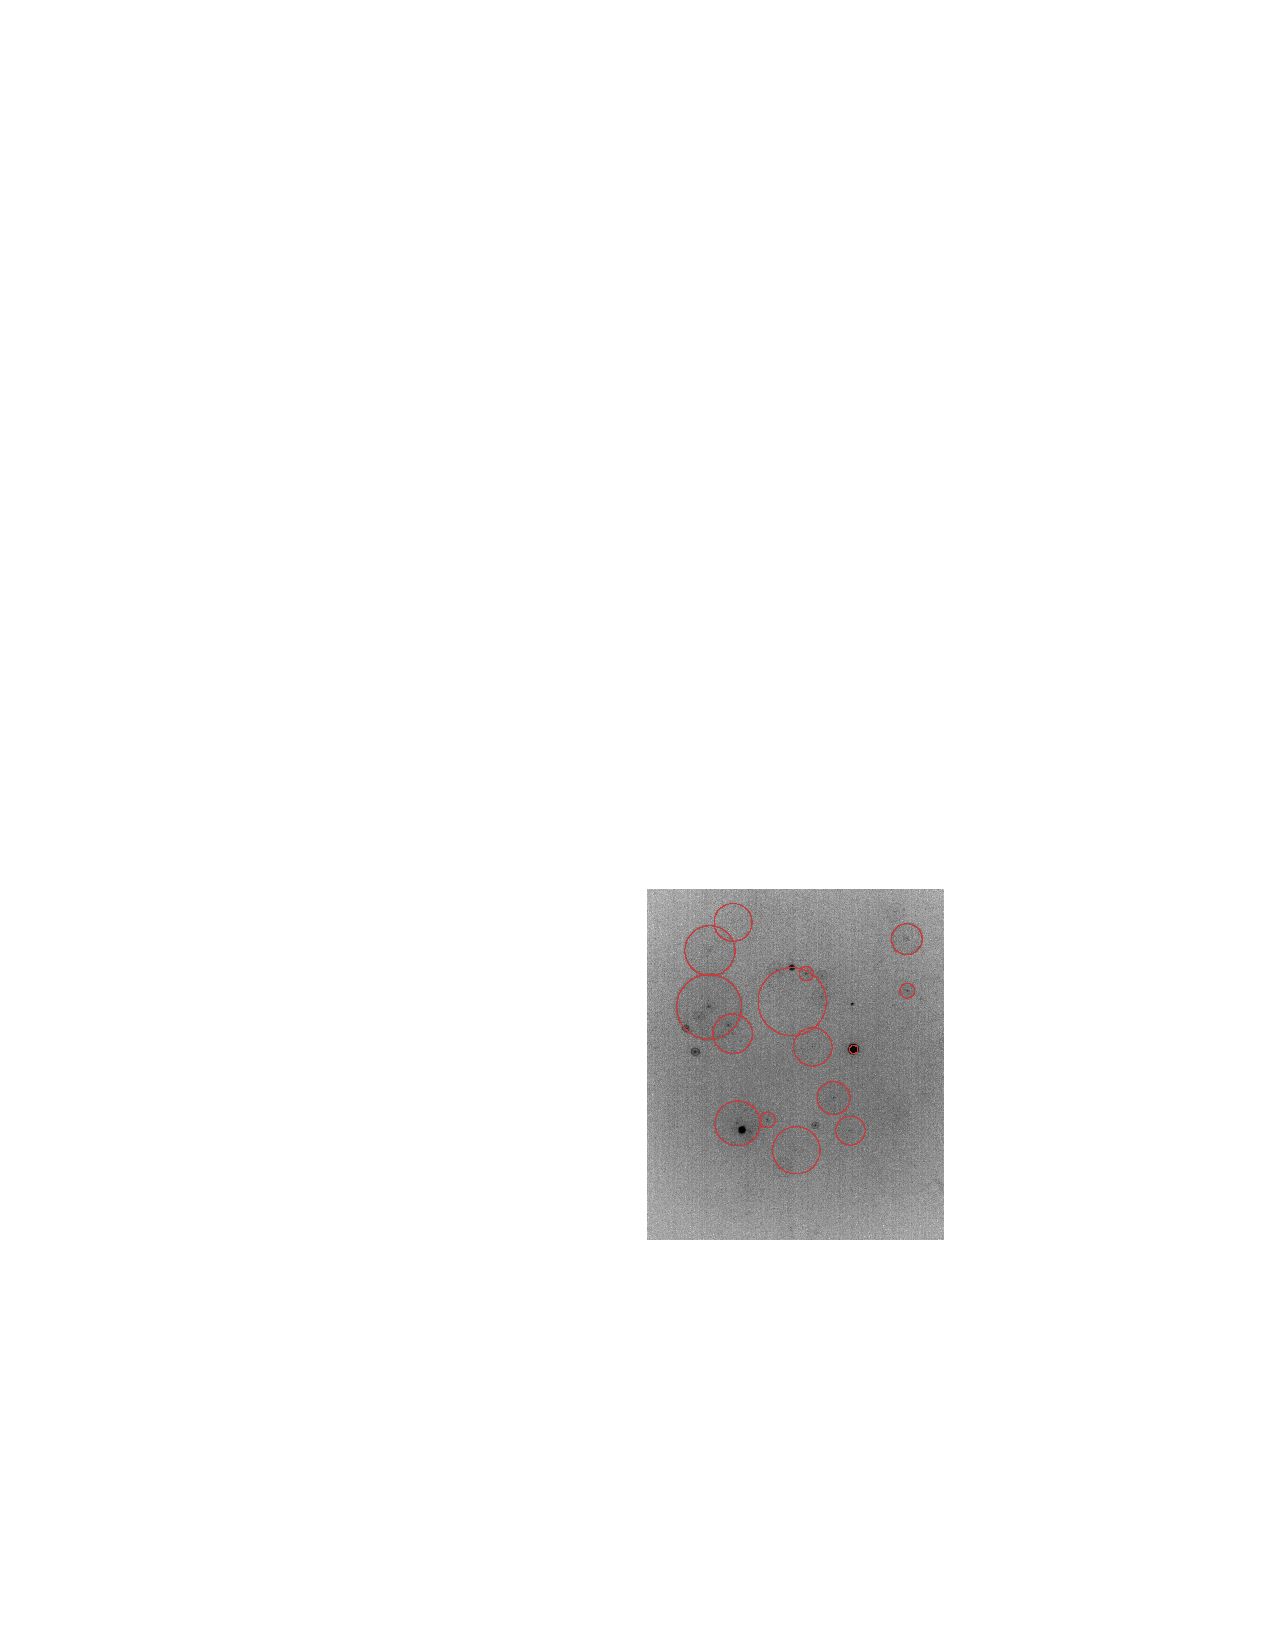
\includegraphics[width=0.35\textwidth]{figs/alex-result.pdf}\qquad
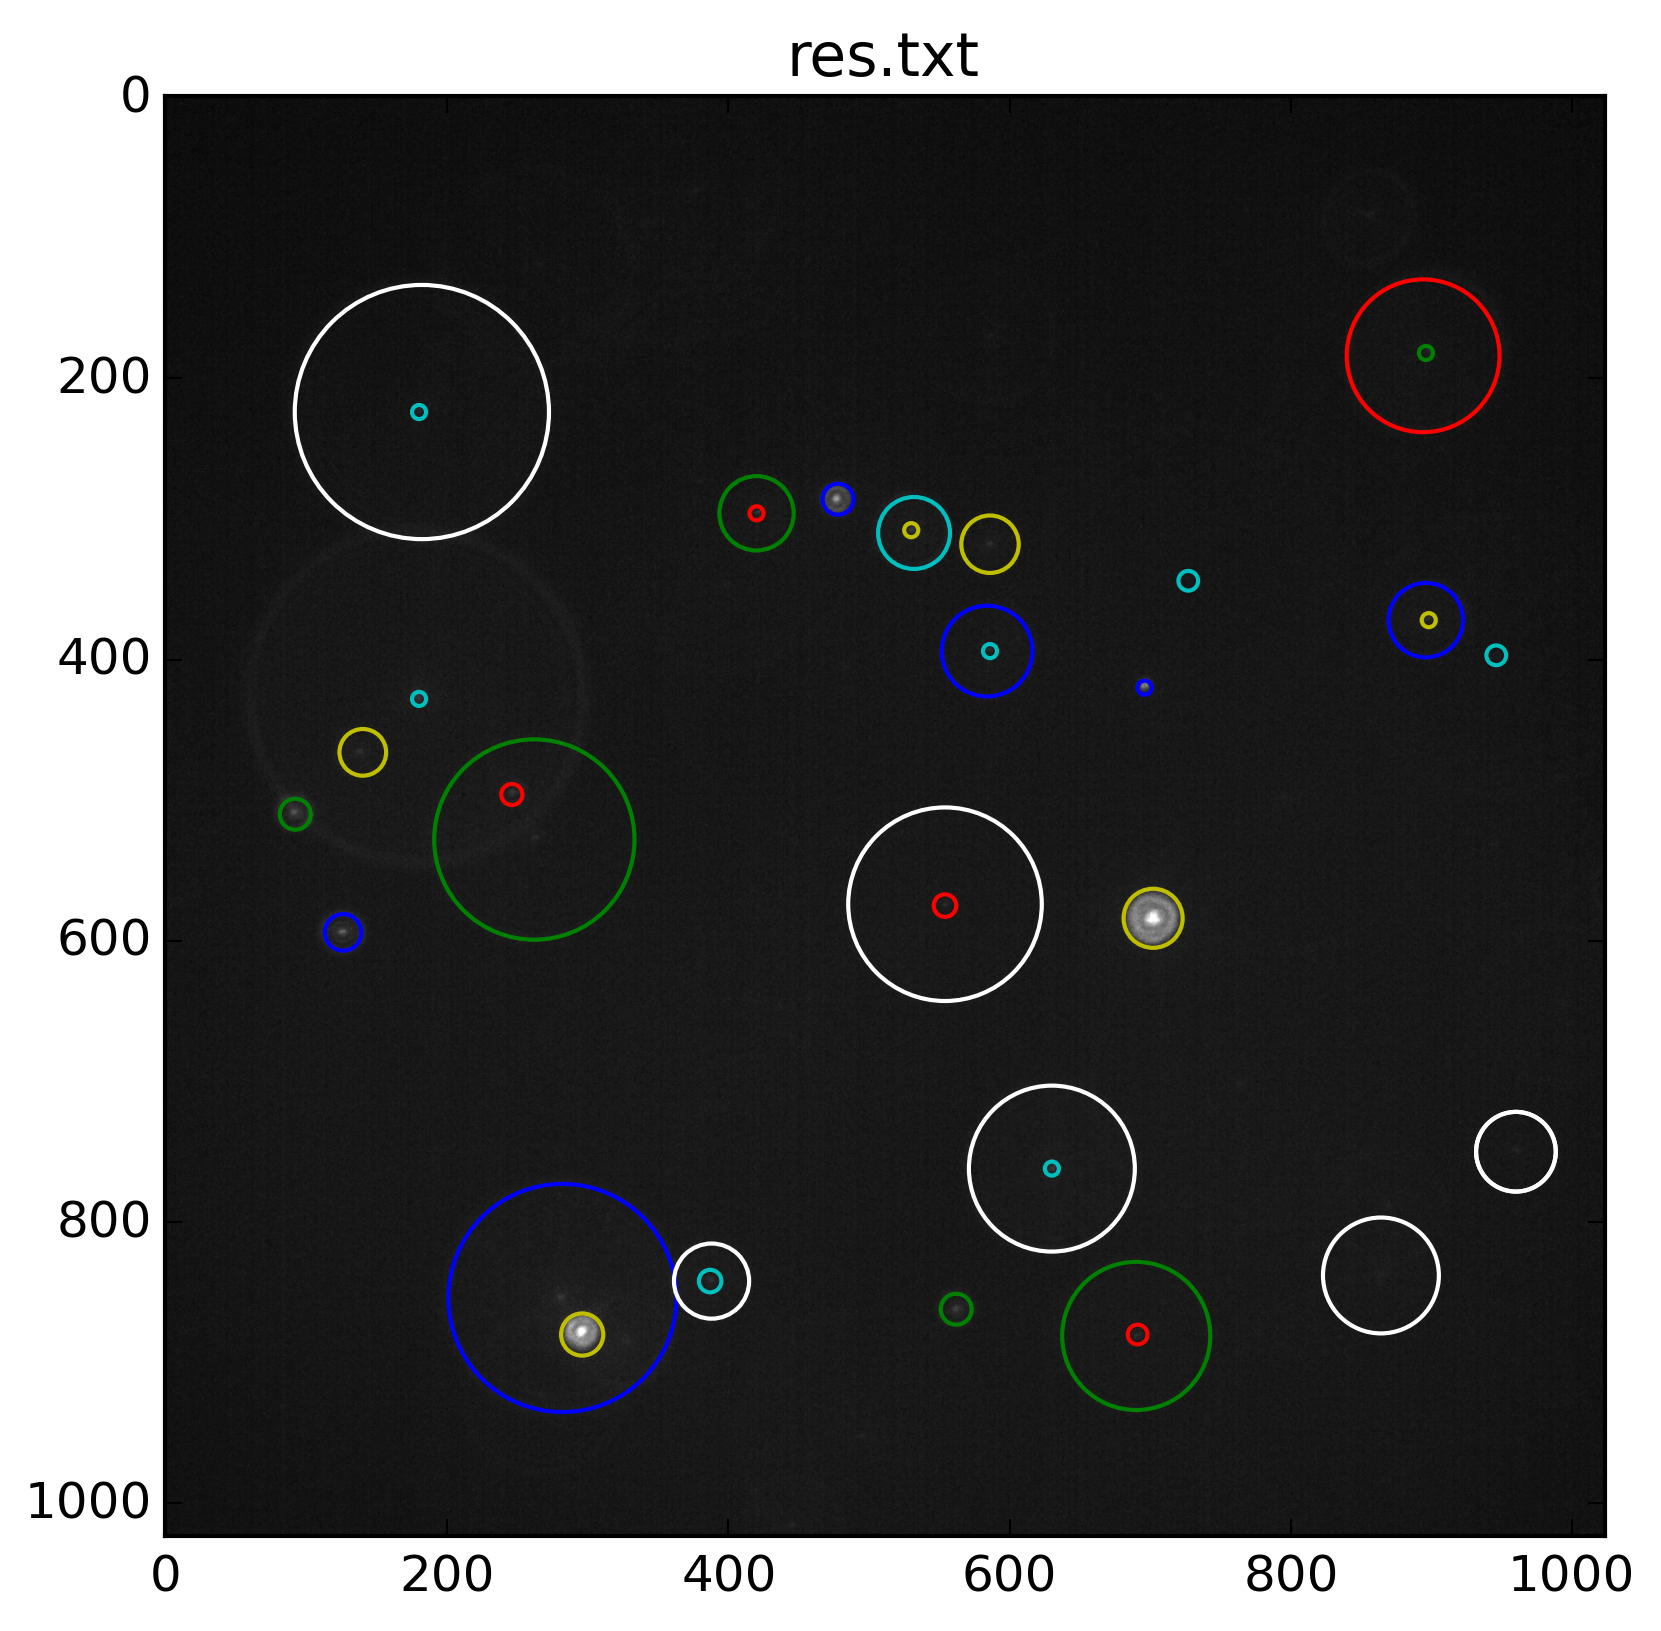
\includegraphics[width=0.35\textwidth]{figs/chuan-res.png}
\label{fig:input}
\caption{quality}
\end{figure}

\section{Hardware and software environment}



\subsection{Experimental setup}



Short description of the setup. Picture of the observation volume. 



Description of reference datasets (put these datasets also to UFO server to allow comparison of algorithms)





\subsection{The UFO Parallel Computing Framework}



Design principles.



Advantages for the developer



Advantages for the algorithm designer



Interface for the user, options for integration





\section{PIV Algorithm}



Describe analysis chain. Block diagram. Profiling.

Display variants of the algorithm as branches.





\subsection{Image pre-processing}



\subsection{Particle detection}



\subsection{Particle properties}



\subsection{Tracking}





\section{Data}



Presentation of the sample datasets. 



Experiments:

\begin{enumerate}

    \item Focus plane shift; the particles are static and the focus plane is shifted continuously. The position of the particles in the plane can be easily calculated. The ring radius can be calibrated by the plane shift.

\end{enumerate}



The datasets are described by following properties. The image properties are obtained by the "ground truth" algorithm described below.

\begin{itemize}

    \item ID, name, description

    \item Optical parameters: perfect/imperfect optics, magnification, laser intensity, particle size, ...

    \item Image properties: Number of frames, frame rate, Number of particles, velocities, SNR

\end{itemize}



//table datasets//





\subsection{Method to obtain ground truth}

For all test datasets the ground truth is calculated automatically (and checked afterwards). The fact that the particles are moving continuously is used to estimate the particle position in each frame (aka time step). 

This is possible with a higher precision than within a single frame.



Procedure:

\begin{enumerate}

    \item calculate rings

    \item calculate trajectories

    \item histogram of number of particle in each trajectory; eliminate all points that do not belong to a trajectory with more than N points (take N from the histogram)

    \item calculate the particle positions for each frame; interpolate missing data; extrapolate one or two time steps at the end of the trajectories

    \item repeat the procedure with a second algorithm and confirm the results

\end{enumerate}





For the focus plane shift datasets further information can be used to check data quality:

\begin{enumerate}

    \item plot x and y coordinates versus time / frame number. Ensure that there is no trend. Calculate mean values for the particle coordinates.

    \item histogram of the radius differences between two frames. Ensure that all radi change equally.

    \item plot radius verse time / frame number. Ensure the the plots are linear. If not there might be no linear ratio between radius and z coordinate or the phase shift was not constant.

    \item calibrate radius of the rings and z coordinate

\end{enumerate}





// histogram: no particle per trajectory //



// plot x,y vs frame no //



// plot r,dr vs frame no //





\section{Results}



\subsection{Precision}



Evaluation of detection efficiency, concerning false positive and false negatives. Compare with 

Ratzenbook 2013.



// plot: Dataset 1 (phase plane shift), UFO-PIV algorithm, Detection propability vs ring size //







\subsection{Performance}



Present different versions of the code.



\begin{itemize}

    \item (1) 4DTracker: MatLab code, ordered filter approach, single core, no optimization, by Wu et. al

    \item (2.1) "FastTracker": ordered filter code, optimized for parallel execution on CPU, by T Habel and A. Lewkowicz

    \item (2.2) "FastTracker": ordered filter code, optimized for parallel execution on GPU, by T Habel and A. Lewkowicz

    \item (3.1) UFO-PIV: Hough transform, optimized for GPU, executed on CPU, by A. Lewkowicz and C. Miao and the UFO-team

    \item (3.2) UFO-PIV: Hough transform, optimized for GPU, executed on GPU (Cluster), by A. Lewkowicz and C. Miao and the UFO-team

\end{itemize}



Comparison of the different codes. Relate to the optimization measures above. 



Measure M1: 2.1 and 3.1 (for comparison do also 2.2 and 3.2) are both optimized. The difference is the better suited algorithm in 3. 



Measure M2: 1 and 2.1 have the same algorithm, but 2.1 used parallel optimization for CPUs. 

Compare with the Ratzenbook 2013 code. They exploit M1 and M2. Run our code 3 on CPU only.

Should we introduce code 3.0 on GPU for this purpose?



Measure M3: Compare 2.1 and 2.2 (or 3.1 and 3.2), same implementation but execution on CPU and GPU. 



Measure M4: Not used currently (my be report experience form PyHST?). (csa)



Measure M5: Execute 3.2 at a GPU cluster. The performance of the execution is limited by the number of GPUs. For the 5 camera setup the demand for GPUs scales by additional factor of 5, that more than 4 GPUs per camera brach seem not feasible. 



Measure M6: Execute 3.1 and 3.2 at different CPUs / GPUs and plot versus the release dates of the GPUs. Add roadmap data from the manufactures. 



Check if some measures can be plotted in the same graph? 









\subsection{Particle management}



Measure M7: Analyse quality of particle detection with quality of the resulting trajectory.

Analyst how many particles are needed in a volume and time slice in relation to the velocity to get a good quality of the flow field.







\section{Conclusion}



The UFO platform is ideal to create workflows with optimized algorithms. 



UFO-PIV code is the fastest code and available online. It can be easily customized for other setups. 



Public high-quality code is crucial of the development of cutting edge experiments in all communities. Only with a common effort maintainable and reliable code can be ensured in the future. 



Online monitoring seems to the feasible, while not completely reached. The group will proceed to develop the first online PIV setup with 3D visualization in a volume of about 100um x 100 um x 100 um.



Future plans, next steps to develop the aimed online monitoring.

 

Scientific GPU computing is affordable and can replace tedious computations for many applications. Beside PIV there are other applications like tomography where GPUs have been successfully used.



Link the the UFO-PIV code repository or website. Publish also the sample dataset used in the article. The UFO-PIV code and the dataset should be stored at GitHUB / zenodo.org with an DOI.







\section{Acknowledgement}



The group of Wu for the initial code 4DTracker.



The UFO framework has been initiated due to UFO Grants and has been developed to universal framework for online monitoring systems for high data-rate since then.





\section{Workplan}



Roadmap: 

\begin{enumerate}

    \item Implement ground truth algorithm. Calculate ground truth for focus plane shift dataset.

    \item Compute with best algorithm and display performance and quality (false positive + negative). Detection probability versus ring size.

    \item Repeat with ground truth calculation with a second algorithm. Validate ground truth. Merge results. 

    \item Compute results with all algorithms and all platforms. Put all relevant data in a spreadsheet.

        Computer name, CPU type, GPU type;

    \item Collect extra table with release data:

        CPU/GPU types; release date; theoretical max performace; 

\end{enumerate}





\section{Methodology} 

For ring detection, we use the circular Hough Transform (CHT).  Since the
defocued ... method, ring edges are thick, fuzzy and have rather low contrast
against the background.  we have skipped the edge detection, apply HT directly
to the input image, following contrast adjustment.  As a result, the HT votes
are contaminated by pixels that does not belong to any shape and are therefore
very noisy. For the purpose of efficiently and reliably sepearte the signal
from noises, we used a likelihood ratio function to filter the votes.  And
later for determining the ring sizes, radical histogram algorithm is used.

\subsection{Pre-processing}
we apply a contrast adjustment, remove background noise would help.
from histogram background noise gaussian distribution, signal in tail
we find the position and width of the histogram peak, and remove all pixels below threadshold
$$s = I_{\mathrm{peak}} + n *\sigma_\mathrm{peak}$$
n is a parameter, which is usally set to 1.

\subsection{Hough Transform: ring templates} 

Circular Hough transform, maps the input image into accumulator space, x, y and
r.  Although the space is continous, in practice it is divided into discrete
cells.  Each cell corrsponds to superpositions of all ring shapes from postions
included in the cell.  We can view the CHT as a approach combining template
matching and HT. We use ring template with various ring size, covolve with
input image. The covolution is used as votes in accumulator space.

We have studied the impacts of ring templates on the voting. For a step fucntion,
..., side slobes. Therefore we use a skewed function..., ..... To account for the
fuzzy egeds, we gaussain shape of the skewed function,...

\subsection{Likelihood ratio}
Hough transform.
common strategy is to apply an edge detection before HT.
Images of micro particles are fuzzy, does not have a crisp edges. 
Signals can be very close to the background.
We imporve the contrast to gain higher SNR instead of edge detection.

\begin{figure}
\centering
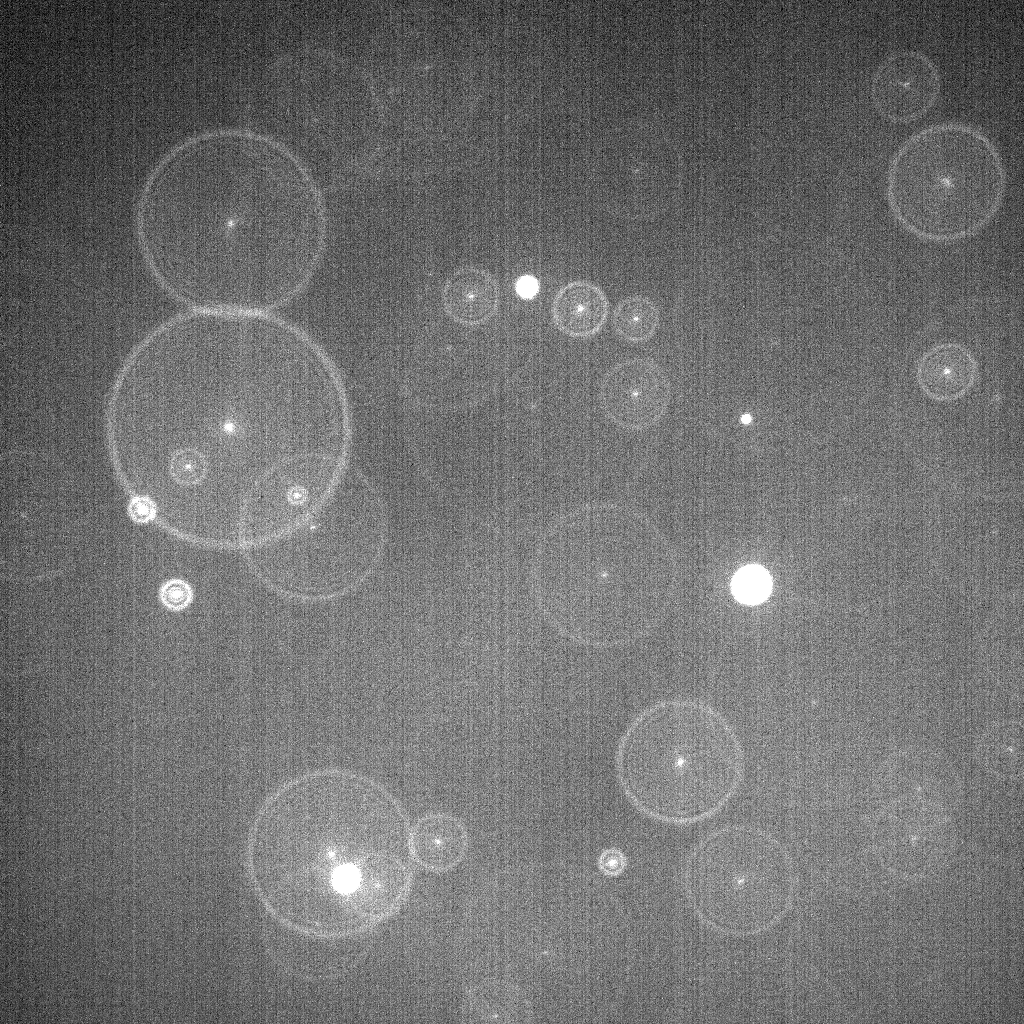
\includegraphics[width=0.35\textwidth]{figs/image1.png}\qquad
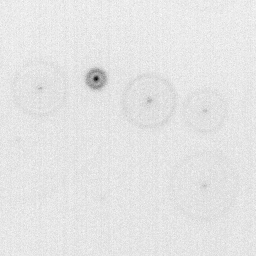
\includegraphics[width=0.35\textwidth]{figs/img0-crop.png}
\label{fig:input}
\caption{Picture captured in experiment.}
\end{figure}


contrast, histogram, singmoid, background fitting

\begin{figure}
\centering
\includegraphics[width=0.25\textwidth]{./figs/img0-crop-contrast.png}
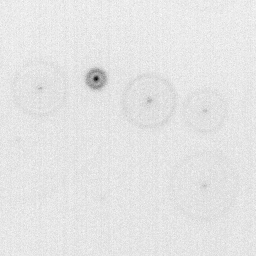
\includegraphics[width=0.35\textwidth]{figs/img0-crop.png}
\end{figure}


Likelyhood function. 
\begin{equation}
    L(\pi_{ij}) = \exp\left( -\frac{1}{\sigma_n^2 } \sum \right)
\end{equation}




\end{document}
